% Solving the Poisson equation with ug4

\documentclass[xcolor=dvipsnames]{beamer}

\usepackage[latin1]{inputenc}
\usepackage{amsmath, amsfonts, amssymb}
\usepackage{graphicx}
\usepackage{color}
\usepackage{setspace}

\usetheme{Copenhagen}
\usecolortheme[named=YellowOrange]{structure}

%\usefonttheme{default}
\usefonttheme {structurebold}
\useinnertheme{default}
\useoutertheme{default}
\setbeamertemplate{headline}[default]

\newcommand*\oldmacro{}%
\let\oldmacro\insertshorttitle%
\renewcommand*\insertshorttitle{%
  \oldmacro\hfill%
  \insertframenumber\,/\,\inserttotalframenumber}

\title
 [ug4: 1st simulation]
 {ug4: Example of a Simulation}
\author [D. Logashenko] {Dmitry Logashenko}
\institute [CEMSE]
{CEMSE, KAUST, Saudi Arabia}
\date [Feb. 2025] {February 2025}

\begin{document}

\frame {\titlepage}

\begin {frame} [t]
\frametitle {Contents}
\tableofcontents
\end {frame}

\section {Numerical solution of elliptic PDEs}

\begin {frame} [t]
\frametitle {Diffusion equation (stationary case)}
$$
 \begin{array} {rcll}
  - \nabla \cdot (\mathbf{D} \nabla u) & = & f, & x \in \Omega \subset \mathbb{R}^2 \\
  u & = & g_D, & x \in \Gamma_D \\
  \mathbf{D} \nabla u \cdot \mathbf{n} & = & 0, & x \in \Gamma_N 
 \end{array}
$$
where
\begin {itemize}
	\item $\mathbf{D} = \mathbf{D} (x) \in \mathbb{R}^2$ is the diffusion tensor,
	\item $f = f (x) \in \mathbb{R}$ are the sources,
	\item $\Gamma_D \cup \Gamma_N = \partial \Omega$, $\Gamma_D \cap \Gamma_N = \emptyset$
		are Dirichlet and Neumann boundaries
	\item $g_D = g_D (x) \in \mathbb{R}$ are the Dirichlet values,
	\item $\mathbf{n}$ is the outer normal.
\end {itemize}

\pause
\vspace {2ex}
(As an exercise for this presentation, we assume that $\mathbf{D} (x) = \mathbf{I}$
but the general case is supported in ug4, too.)
\end {frame}

\begin {frame} [t]
\frametitle {Numerical solution of the PDE}
\vspace {-2ex}
The classical approach includes the following phases:
\begin {enumerate}
	\item {\color{red} Discretization}: The continuum domain $\Omega \subset \mathbb{R}^d$
		is covered by a {\color{blue} grid} $\Omega_h$, $u$ is approximated by a
		{\color{blue} grid function} $u_h$ from a finite-dimensional space, the differential
		operator is replaced by an {\color{blue} algebraic} operator between finite-dimensional spaces.
		Therefore, the PDE is converted to a {\color{blue} large sparse system of algebraic equations}. \\
		Keywords: FD, FE, FV discretization, etc.
	\pause
	\item {\color{red} Solution of the algebraic system}: The {\color{blue} solver} should
		be sufficiently efficient for the system of this size. It should profit from the sparsity,
		hardware architecture etc. \\
		Keywords: CG, BiCGStab etc. iterations, GMG, AMG preconditioners,
		ILU, GS smoothers etc.
	\pause
	\item {\color{red} Post-processing}: {\color{blue} Visualization} or extraction of specific data. This may
		include interpolation, quadrature etc. Normally, this assumes some output
		of the solution.
\end {enumerate}
\end {frame}

\section {Discretization}

\begin {frame} [t]
\frametitle {Shape functions}
Discrete solution $u_h$ is represented as
$$
 u_h (x) = \sum_{i = 1}^{N} u_i \lambda_i (x),
$$
where $\lambda_i: \Omega \to \mathbb{R}$ are continuous piecewise linear functions with
\centerline {$\lambda_i (x_i) = 1, \quad \lambda_i (x_j) = 0 \quad (j \ne i)$ (``hat functions'').}

\vspace {2ex}
\centerline {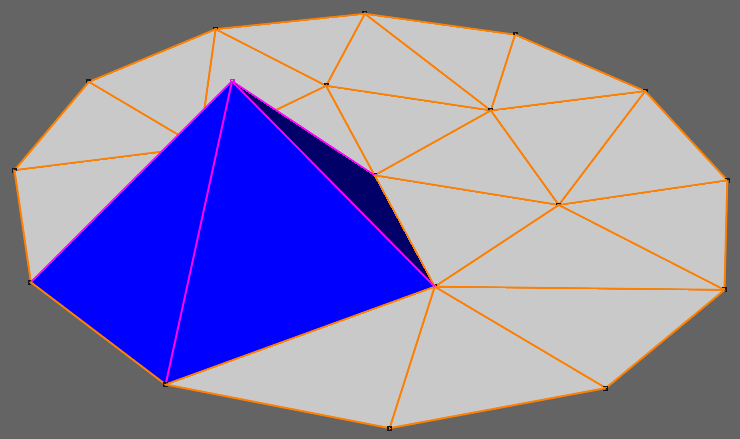
\includegraphics [width = 0.5\textwidth] {Circle-phi.png}}

\centerline {$u_i$: ``degrees of freedom''}
\end {frame}

\begin {frame} [t]
\frametitle{Bilinear shape functions}
are used for quadrilaterals:
\centerline {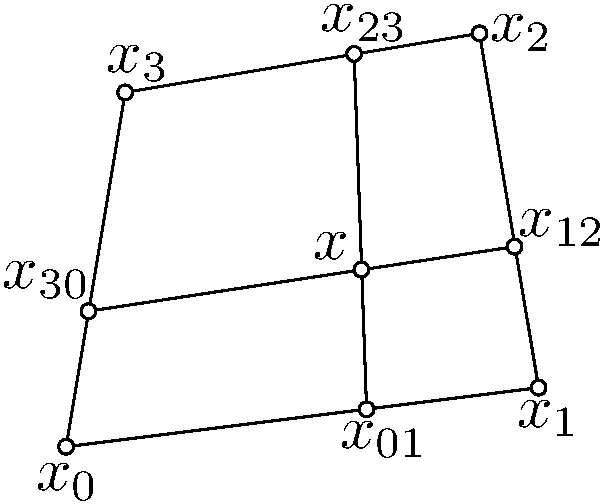
\includegraphics [width = 0.5\textwidth] {bilinear-geometric.pdf}}
\centerline {(linear along every of the presented lines)}
\end {frame}

\begin {frame} [t]
\frametitle{Finite Volumes: Dual grid}
\centerline{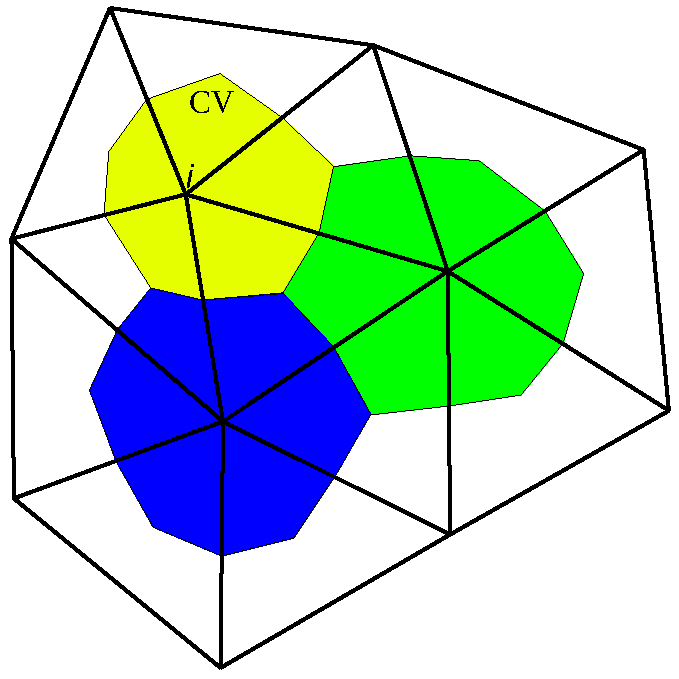
\includegraphics [width=0.6\textwidth] {FV-Elem-Donald-Scheme.pdf}}
\only<1>
{%
\centerline{Donald Diagrams: Connect the midpoints.}
}%
\only<2>
{%
\centerline {$\displaystyle - \nabla \cdot (\mathbf{D} \nabla u) = f$}
}%
\only<3>
{%
\centerline {$\displaystyle - \int_{\mathrm{CV}} \nabla \cdot (\mathbf{D} \nabla u) \, dx = \int_{\mathrm{CV}} f \, dx$}
}%
\only<4>
{%
\centerline {$\displaystyle - \int_{\mathrm{\partial CV}} (\mathbf{D} \nabla u) \cdot \mathbf{n} \, dx = \int_{\mathrm{CV}} f \, dx$}
}%
\end {frame}

\begin {frame} [t]
\frametitle{Finite Volume Finite Element Method}
\centerline{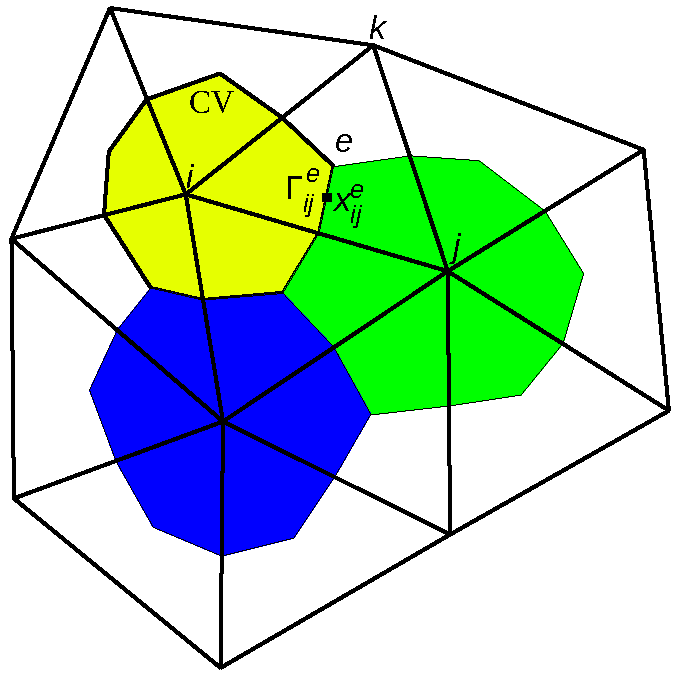
\includegraphics [width=0.6\textwidth] {FV-Elem-Donald.pdf}}
\only<1>
{%
\centerline{$\displaystyle u_h = \sum_i u_i \lambda_i$: a piecewise linear function}
}%
\only<2>
{%
\centerline{$\displaystyle \nabla^e u_h = \sum_i u_i \nabla^e \lambda_i$: a linear combination}
}%
\only<3>
{%
\centerline{$\displaystyle - \sum_{e \ni x_i} \sum_{j \ne i} | \Gamma^e_{ij} | \mathbf{D}^e_{ij} \nabla^e u_h \cdot \mathbf{n}^e_{ij} = | \mathrm{CV}_i | f_i$}
}%
\end {frame}

\begin{frame} [t]
\frametitle {Neumann Boundary Conditions}
\centerline{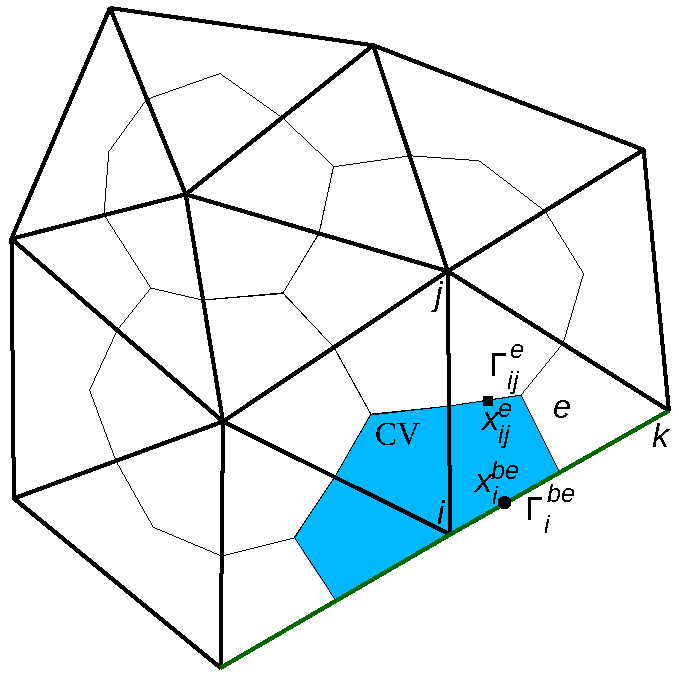
\includegraphics [width=0.6\textwidth] {FV-Elem-Donald-bnd.pdf}}
\centerline{%
$
 \left .  \mathbf{D} \nabla u \cdot \mathbf{n} \right |_{\Gamma_N} = g_N: \,
 \displaystyle
 - \sum_{e \ni x_i}
  \bigl (
   \sum_{j \ne i} | \Gamma^e_{ij} | d^e_{ij} \nabla^e u_h \cdot \mathbf{n}^e_{ij}
   +
   | \Gamma^{be}_{i} | g_{N,i}
  \bigr )
 = | \mathrm{CV}_i | f_i
$%
}
\end{frame}

\begin {frame} [t]
\frametitle {``Local'' and ``global'' assembling}
\vspace {-2ex}
\begin {itemize}
	\item One computes the contributions of {\color{blue} every full-dimensional grid element}.
		The cycle over all these elements and summing up the contributions is referred to as
		``global assembling'' (``{\color{blue} domain discretization}'' in ug4). This
		part is mostly problem and discretization independent.
	\pause
	\item In every full-dimensional grid element, one uses the shape functions and the
		geometrical information to evaluate the {\color{blue} local contributions}. These computations
		are called ``local assembling'' (``{\color{blue} element discretization}'' in ug4).
	\pause
	\item The standard ``{\color{blue} domain discretization}'' is implemented in {\color{blue} ugcore}.
		It profits from the special representation of the grid topology as well as from
		the usage of the class templates.
	\pause
	\item ``{\color{blue} Element discretizations}'' are problem-specific and typically implemented
		in the {\color{blue} plugins}. The ConvectionDiffusion plugin implements several local assembling
		routines.
\end {itemize}
\end {frame}

\section {Geometries and grids in ug4}

\begin {frame} [t]
\frametitle {Geometries and grids in ug4}
\begin {itemize}
	\item Any spatial domain in ug4 is represented by a {\color{blue} coarse mesh} and (if necessary)
		{\color{blue} projectors} of boundary patches. This information is kept in the ugx-file and
		called {\color{blue} ``the geometry''} (or ``the grid'').
	\pause
	\item When loaded, this grid is {\color{blue} refined} (i.e. its elements are subdivided). By this,
		one creates a grid with the desired mesh size. Thus (for the specified refinement
		strategy) the mesh size of the grid is characterized by the {\color{blue} refinement
		(or grid) level}.
	\pause
	\item During the refinement, the new boundary grid nodes {\color{blue} are projected} to the actual boundary.
	\pause
	\item The sequence of the consequently refined grids form the grid hierarchy --- the s.c.
		{\color{blue} multigrid}. This hierarchy is stored and can be used by some solvers
		(e.g. geometrical multigrid method).
\end {itemize}
\end {frame}

\begin {frame} [t]
\frametitle {Unstructured grid hierarchy: Example}
\vspace {-1ex}
\only<1>{\centerline {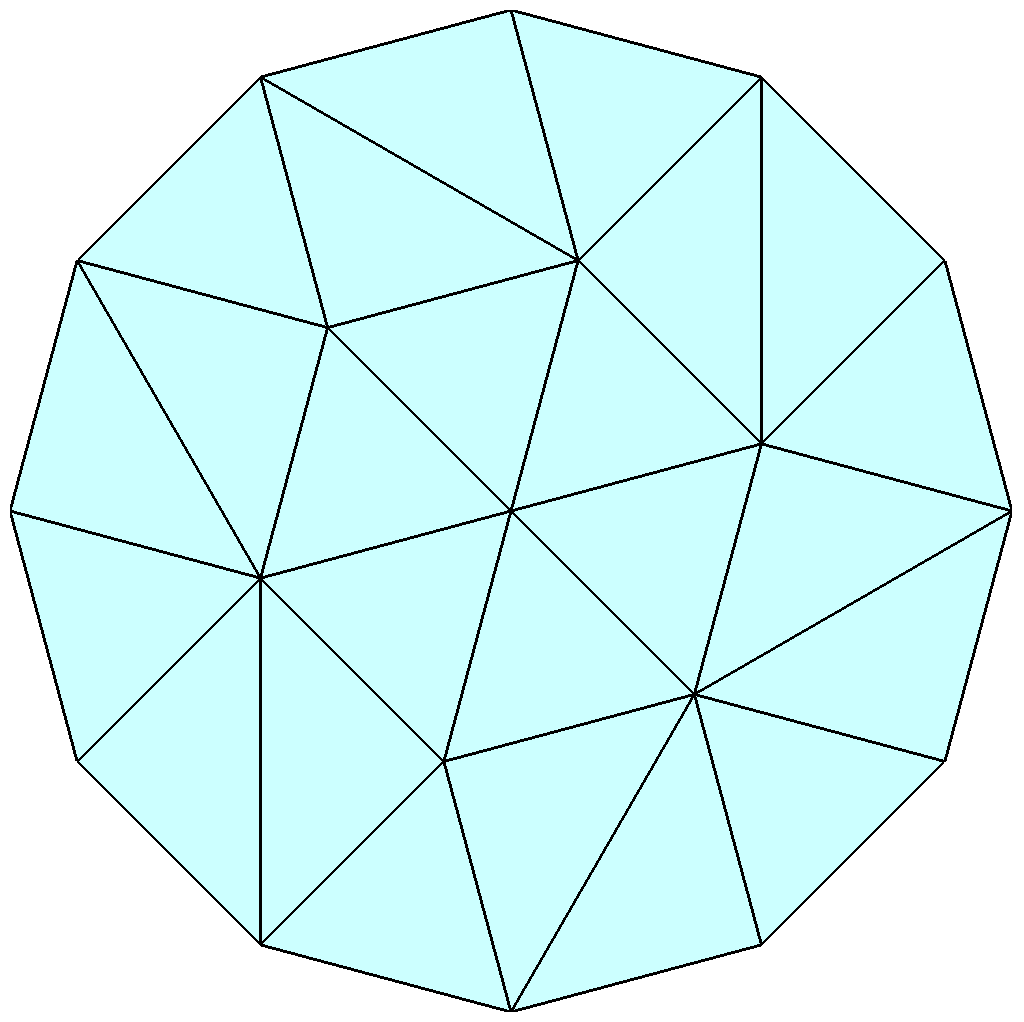
\includegraphics [width = 0.7\textwidth] {Circle-lev0.png}}\centerline{Grid level 0}}%
\only<2>{\centerline {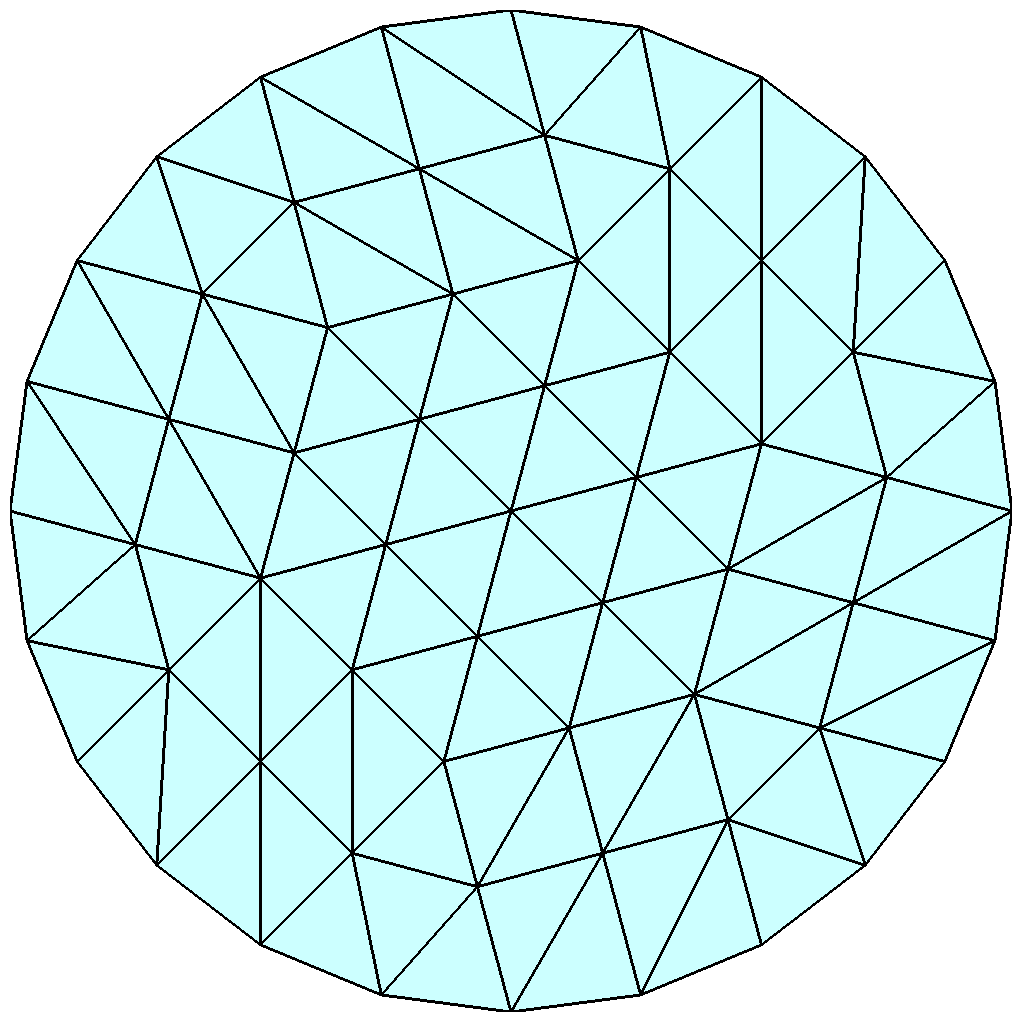
\includegraphics [width = 0.7\textwidth] {Circle-lev1.png}}\centerline{Grid level 1}}%
\only<3>{\centerline {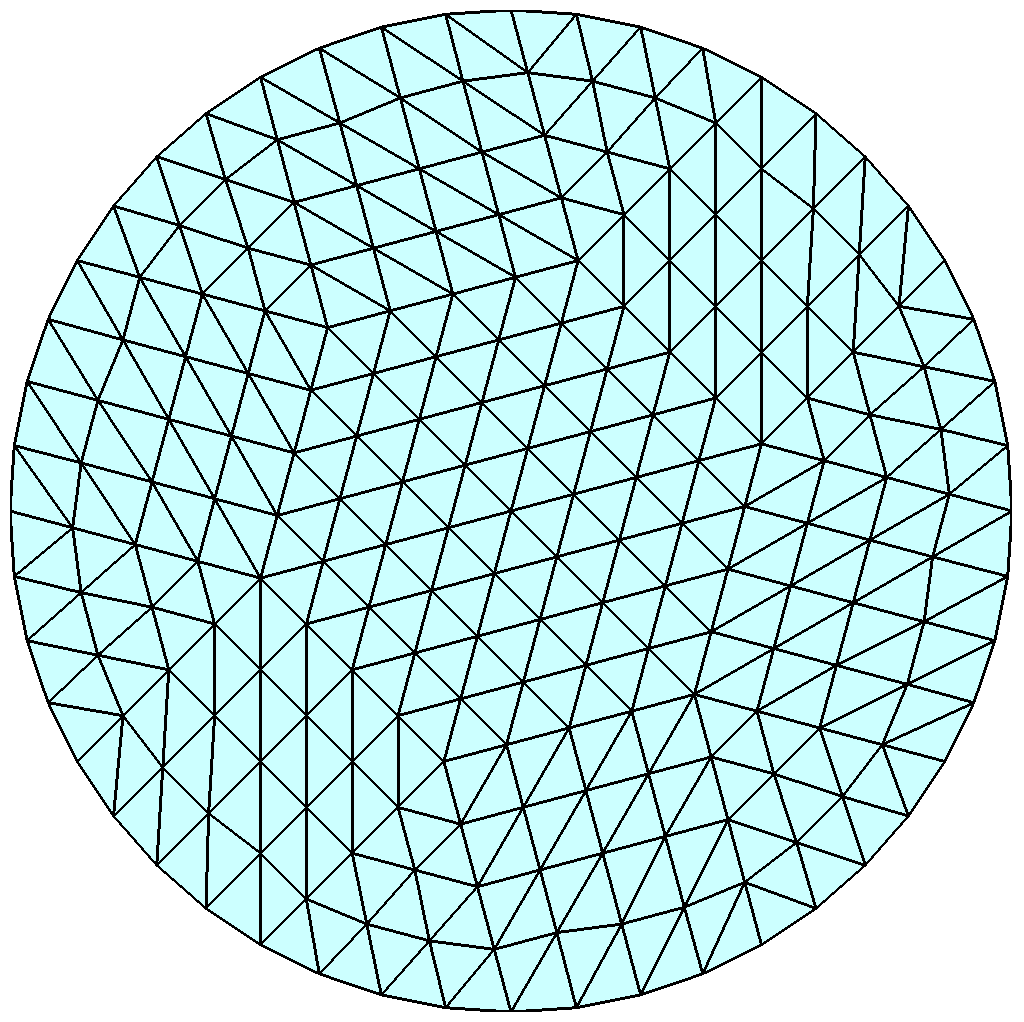
\includegraphics [width = 0.7\textwidth] {Circle-lev2.png}}\centerline{Grid level 2}}%
\end {frame}

\begin {frame} [t]
\frametitle {Grid elements}
An $d$-dimensional grid consists of {\color{blue} grid objects} with dimensionalities
$0 \dots d$:
\begin {itemize}
	\item 0d: {\color{blue} Vertices}
	\item 1d: {\color{blue} Edges} (segments of straight lines)
	\item 2d: {\color{blue} Faces} ({\color{blue} triangles} and {\color{blue} quadrilaterals})
	\item 3d: {\color{blue} Volumes} ({\color{blue} tetrahedra}, {\color{blue} hexahedra},
		{\color{blue} prisms}, {\color{blue} pyramids} and {\color{blue} octahedra})
\end {itemize}
(Sides of $d$-dimensional objects are $(d-1)$-dimensional objects.)

\pause
\vspace {1ex}
A subset of all grid objects in a geometry is referred to as {\color{blue} subset}. Subsets
are used for ex. to specify boundary conditions or to separate parts of the domain with
different properties (model coefficients etc.).
\end {frame}

\section {A simple script}

\begin {frame} [t]
\frametitle {A simple script}
\vspace{-2ex}
Solution of the Poisson equation on a square:

\vspace {1ex}
{\color{blue} ugshell -ex poisson\_err.lua -numRefs 5}

{\tiny \color{red} (Prepend appropriate paths!)}

\pause
\vspace {1ex}
A LUA script creates the objects of classes implemented in C++ and calls their methods.

\pause
\vspace {1ex}
Important notions:
\begin {itemize}
	\item {\color{blue} ApproximationSpace} assigns DoFs to the grid objects and
		defines the interpolation of the DoFs (i.e. provides the shape functions).
	\item {\color{blue} GridFunction} stores the DoFs and references the ApproximationSpace.
\end {itemize}

\pause
\vspace {1ex}
For convinience, ug4 provides the LUA utilities that help to initialize the domain,
construct the solvers etc.
\end {frame}

\begin {frame} [t]
\frametitle {Discretization and solver objects}
\centerline {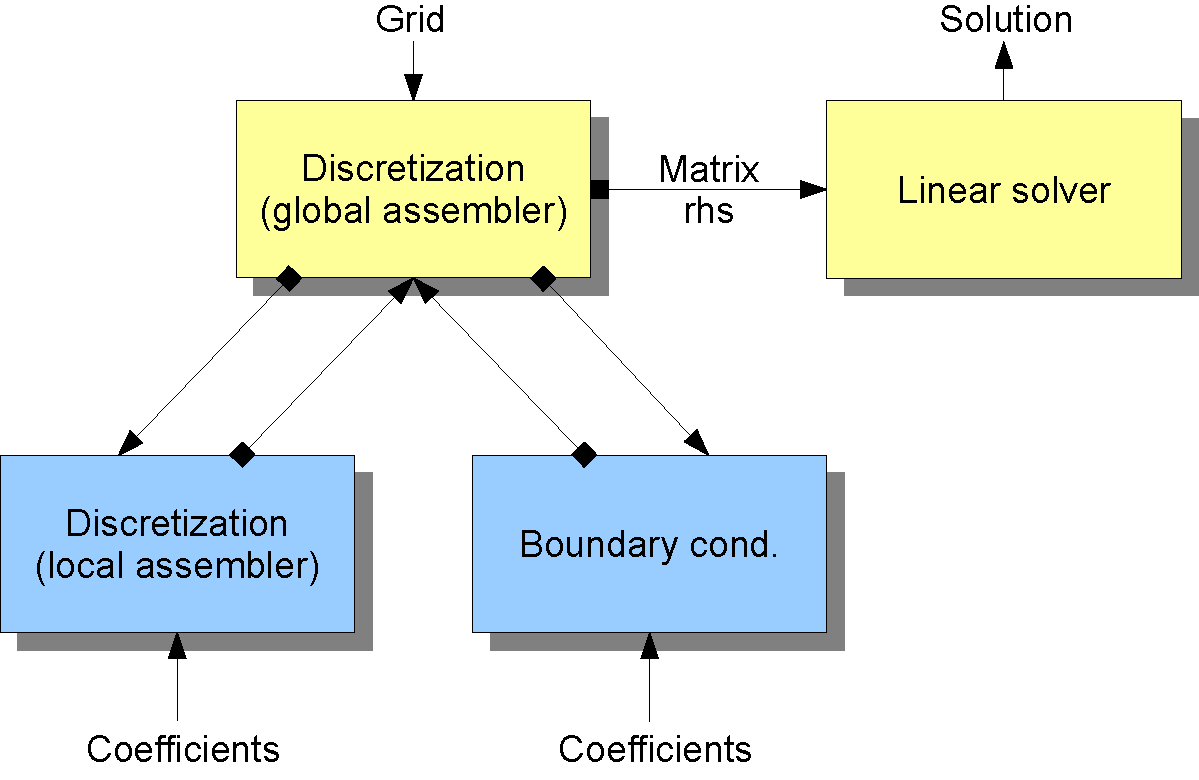
\includegraphics [width=1.05\textwidth] {Discretization}}
\end {frame}

\section {Conclusions}

\begin {frame} [t]
\frametitle {Thank you for your attention!}
We considered:
\begin {itemize}
	\item Basic ideas of the FV discretization of the Poisson equation
	\item Representation of domain geometries in ug4
	\item LUA scripts in ug4
	\item Setting up discretizations in ug4
\end {itemize}

\vspace{3ex}
Supplementary scripts:
\begin {itemize}
	\item my\_1st.lua --- grid refinement, initialization of a grid function
	\item my\_2nd.lua --- the same but with LUA utilities
	\item poisson\_err.lua --- solution of the Poisson equation on a square,
		computation of the discretization error
\end {itemize}
\end {frame}

\end{document}

% End of File
